\documentclass[accentcolor=tud0b,12pt,paper=a4]{tudreport}

\usepackage[utf8]{inputenc}
\usepackage{ngerman}
\usepackage{parcolumns}
\usepackage{parskip}

% include wkhtmltopdf stuff
\usepackage{pdfpages}

% code review checklist
\usepackage{enumerate}

% pandoc

\usepackage{longtable}
\usepackage{booktabs}
% fix for pandoc 1.14
\providecommand{\tightlist}{%
  \setlength{\itemsep}{0pt}\setlength{\parskip}{0pt}}
\usepackage{framed}
\usepackage{listings}
\usepackage{color}

\usepackage{listings}
\lstset{
basicstyle=\small\ttfamily,
columns=flexible,
breaklines=true
}

\usepackage{fancyvrb}
\definecolor{shadecolor}{RGB}{238,238,238}

\DefineVerbatimEnvironment{Highlighting}{Verbatim}{commandchars=\\\{\}}
%\newenvironment{Highlighting}{\begin{lstlisting}}{\end{lstlisting}}
% Add ',fontsize=\small' for more characters per line
\newenvironment{Shaded}{\begin{shaded*}\scriptsize}
 {\end{shaded*}}

\newcommand{\KeywordTok}[1]{\textcolor[rgb]{0.00,0.44,0.13}{\textbf{{#1}}}}
\newcommand{\OperatorTok}[1]{\textcolor[rgb]{0.00,0.44,0.13}{\textbf{{#1}}}}
\newcommand{\DataTypeTok}[1]{\textcolor[rgb]{0.56,0.13,0.00}{{#1}}}
\newcommand{\DecValTok}[1]{\textcolor[rgb]{0.25,0.63,0.44}{{#1}}}
\newcommand{\BaseNTok}[1]{\textcolor[rgb]{0.25,0.63,0.44}{{#1}}}
\newcommand{\FloatTok}[1]{\textcolor[rgb]{0.25,0.63,0.44}{{#1}}}
\newcommand{\CharTok}[1]{\textcolor[rgb]{0.25,0.44,0.63}{{#1}}}
\newcommand{\StringTok}[1]{\textcolor[rgb]{0.25,0.44,0.63}{{#1}}}
\newcommand{\CommentTok}[1]{\textcolor[rgb]{0.38,0.63,0.69}{\textit{{#1}}}}
\newcommand{\OtherTok}[1]{\textcolor[rgb]{0.00,0.44,0.13}{{#1}}}
\newcommand{\AlertTok}[1]{\textcolor[rgb]{1.00,0.00,0.00}{\textbf{{#1}}}}
\newcommand{\FunctionTok}[1]{\textcolor[rgb]{0.02,0.16,0.49}{{#1}}}
\newcommand{\RegionMarkerTok}[1]{{#1}}
\newcommand{\ErrorTok}[1]{\textcolor[rgb]{1.00,0.00,0.00}{\textbf{{#1}}}}
\newcommand{\NormalTok}[1]{{#1}}
%\EndDefineVerbatimEnvironment{Highlighting}


% clickable hyperlinks in the table of contents
\usepackage{hyperref}

\usepackage{listings}

\newcommand{\titlerow}[2]{
  \begin{parcolumns}[colwidths={1=.15\linewidth}]{2}
    \colchunk[1]{#1:}
    \colchunk[2]{#2}
  \end{parcolumns}
  \vspace{0.2cm}
}

\title{Entwicklung eines adaptiven Chat-Systems}
\subtitle{Qualitätssicherungsdokument}
\subsubtitle{%
  \titlerow{Gruppe 9}{%
    Johannes Lauinger <johannes.lauinger@gmail.com>\\
    Jonas Mönnig <jonas.moennig@gmx.de>\\
    Mattias Hofmann <chaterMH@web.de>\\
    Maximilian Weller <maximilian.weller@stud.tu-darmstadt.de>\\
    Simon-Konstantin Thiem <simon-konstantin.thiem@stud.tu-darmstadt.de>}
  \titlerow{Teamleiter}{Benjamin Tumele <B.Tumele@gmx.de>}
  \titlerow{Auftraggeber}{%
    Alexander Frömmgen <froemmge@dvs.tu-darmstadt.de>\\
    Fachgebiet Datenbanken und Verteilte Systeme\\
    Fachbereich Informatik\\
    Jens Heuschkel <jens.heuschkel@tk.informatik.tu-darmstadt.de>\\
    Fachgebiet Telekooperation\\
    Fachbereich Informatik}
  \titlerow{Abgabedatum}{06.07.2015}}
\institution{Bachelor-Praktikum SoSe~2015\\Fachbereich Informatik}

\begin{document}

  \maketitle
  \tableofcontents

  \chapter{Einleitung}
  
Mobile Kommunikation ist in der heutigen Zeit selbstverständlich geworden. Wir verlassen uns mehr und mehr darauf, auch von unterwegs jederzeit Nachrichten senden und empfangen zu können. Hierfür wird zum größten Teil das Handynetz verwendet.

Problematisch ist dabei, dass das Mobilfunknetz auf einen bestimmten Frequenzbereich beschränkt ist und daher nicht beliebig viele Nachrichten parallel verschickt werden können. Insbesondere bei Veranstaltungen, bei denen sich sehr viele Menschen auf relativ geringem Platz versammeln, kommt es häufig zu Netzausfällen. Ein Beispiel ist das Darmstädter Schlossgrabenfest, auf dem in den letzten Jahren ca. 100 000 Menschen anwesend waren.

Ziel unseres Projekts ist es, eine Nachrichtenplattform für solche Extremsituationen zu schaffen. Diese soll zusätzlich zur aktuell bereits häufig eingesetzten Möglichkeit, über eine Client-Server-Infrastruktur zu kommunizieren, ein Peer-to-Peer Netzwerk einsetzen. Dies bedeutet, dass die Geräte untereinander ein Netzwerk aufbauen, welches unabhängig von zentralen Netzen funktioniert, und über das Nachrichten verschickt werden können. Kann eine Nachricht nicht unmittelbar zum Empfänger geschickt werden, können weitere Geräte die Nachricht weiterleiten, bis sie am Ziel ankommt.

Die App soll sich in ihrem Funktionsumfang an verbreiteten Messenger-Anwendungen wie zum Beispiel WhatsApp orientieren. Vorerst beschränken wir uns jedoch auf einfache Textnachrichten in Chats mit nur einem Kommunikationspartner. Außerdem wird die App zunächst nur für Android entwickelt.


  \chapter{Qualitätsziele}
  
In Zusammenarbeit mit unseren Auftraggebern haben wir beschlossen, bei der Entwicklung der Anwendung besonders auf Wartbarkeit, Korrektheit und Robustheit zu achten. Im Folgenden sollen nun diese Qualitätsziele und die Maßnahmen zur Sicherstellung genauer vorgestellt werden.

\section{Wartbarkeit durch Codequalität}
Im Rahmen des Projekts konzentrieren wir uns auf Wartbarkeit der Anwendung durch hohe Codequalität. Diese ist nötig, da unsere Auftraggeber die fertige App nächstes Jahr auf dem Schlossgrabenfest einsetzen wollen, um Daten über die Ausfallsicherheit von Netzen zu sammeln und sie dafür möglicherweise weiterentwickeln müssen.

\textbf{Checkstyle}\\
Zur Sicherstellung der hohen Codequalität ist es unter anderem wichtig, auf Lesbarkeit und geringe Codekomplexität zu achten. Dabei unterstützt uns das statische Codeanalysetool Checkstyle. Checkstyle überprüft den Code auf die Einhaltung verschiedenster Programmierrichtlinien und generiert automatisch Berichte. Besonderen Fokus beim Auswerten der Berichte legen wir dabei auf die von Checkstyle errechneten Codemetriken, da diese in direktem Zusammenhang zur Codekomplexität, und daher zur Wartbarkeit stehen. Die Javadoc-Überprüfungen von Checkstyle führen wir jedoch nicht aus, da die Auftraggeber keinen Wert auf ausführliches Javadoc legen.
    
Die Ausführung von Checkstyle stellen wir durch die Integration in das Continuous-Integration-Tool Jenkins sicher. Damit werden die Berichte automatisch bei jedem Push in das Git-Repostitory erstellt, und sind für jeden einsehbar. Sollten Probleme, beispielweise hohe Komplexität oder schlechter Programmierstil, auftreten, werden diese innerhalb von zwei Tagen durch den Verursacher behoben. Dieser ist am letzten Commit eindeutig ersichtlich.
    
\textbf{Code Reviews}\\
Weiterhin führen wir ab dem vierten Sprint Meeting regelmäßig alle zwei Wochen zusammen mit den Auftraggebern Code Reviews durch. Dabei wenden wir den Over-the-Shoulder-Ansatz an. Das bedeutet, dass unsere Auftraggeber sich den Code von einem Entwickler erläutern lassen und Anmerkungen und Fragen einbringen. So werden einerseits Schwächen aufgedeckt und behoben, was unter anderem die Codequalität unterstützt, als auch die Wartbarkeit im Allgemeinen gesteigert und die Zufriedenheit der Auftraggeber erhöht, da diese direkten Einfluss auf den Code haben.
    
Bei den Code Reviews setzen wir eine Checkliste ein, um sicherzustellen, dass der Ablauf des Reviews formal korrekt abläuft. Diese Checkliste stellt gleichzeitig eine Dokumentation und einen Beleg für die Durchführung der Maßnahme dar. Gefundene Probleme werden von dem Entwickler innerhalb des nächsten Sprints behoben, der die entsprechende Funktion implementiert hat.
    
\textbf{Dokumentation}\\
Zuletzt erarbeiten und pflegen wir eine gute technische Dokumentation über die Designentscheidungen und den Aufbau des Codes. Diese wird nicht im Code selbst geführt, sondern als externe Datei im Repository. Fügt ein Entwickler eine neue Funktionalität hinzu oder ändert das aktuelle Design, dokumentiert er diese umfassend.
    
Alle zwei Wochen führen wir im Team gemeinsam ein Review der Dokumentation durch, bei dem sichergestellt wird, dass alle Funktionalitäten ausreichend dokumentiert sind. Ist dies nicht der Fall, ergänzt der Entwickler, der das entsprechende Feature implementiert hat, die Dokumentation bis zum nächsten Review.
    
Durch die Dokumentation wird Wissen im Team an zentraler Stelle gesammelt. Damit verhindern wir zum Beispiel, bereits aus guten Gründen verworfene Entscheidungsmöglichkeiten erneut in Betracht zu ziehen. Weiterhin wird später Entwicklern, die neu in das Team kommen, die Einarbeitung in das Projekt erleichtert.

\section{Korrektheit}
Da die Benutzer der App potenziell wichtige Nachrichten versenden, verlassen sie sich auf die korrekte Funktionsweise der Anwendung. Wir führen entsprechend Maßnahmen durch, um beispielsweise die korrekte Speicherung von Nachrichten und Kontakten sowie die fehlerfreie Verschlüsselung und Übertragung von Nachrichten zu garantieren.
  
\textbf{Automatisierte Tests}\\
Zur Sicherstellung der Korrektheit führen wir regelmäßige automatisierte Tests mit JUnit durch. Die Ausführung der Tests in Jenkins integriert. Wir testen die Packages helper, data und models. Die Klassen für das UI und die Netzwerkkommunikation testen wir dagegen manuell, da dafür schlecht simulierbare Benutzereingaben bzw. mehrere Geräte notwendig sind.
    
Um einzelne Funktionen isoliert testen zu können, setzen wir das Mocking-Framework Mockito ein. Die Testabdeckung messen wir mit dem Werkzeug EclEmma.

Fügt ein Entwickler eine Funktion hinzu, welche automatisiert testbar ist, schreibt er auch einen JUnit Test dafür. Die Ausführung der Tests wird durch Jenkins sichergestellt. Schlägt ein Test fehl, behebt der verantwortliche Entwickler den Fehler. Dieser ist anhand des letzten Commits ersichtlich. Die Tests müssen innerhalb von zwei Tagen wieder bestanden werden.
    
\textbf{FindBugs}\\
Weiterhin setzen wir das statische Codeanalysetool FindBugs ein, um Fehler im Code frühzeitig zu entdecken. FindBugs ist ebenfalls in Jenkins integriert, sodass bei jedem Push ins Repository automatisch in Bericht erstellt wird, der manuell abgerufen wird. Werden Fehler gefunden, behebt diese ebenfalls der durch die History ersichtliche Entwickler, der den Fehler produziert hat innerhalb von zwei Tagen.

\section{Robustheit}
Da die App für Situationen entwickelt wird, in denen die herkömmlichen Funknetzwerke bereits nicht mehr verfügbar sind, muss sie besonders robust funktionieren. Bei einer großen Anzahl von Geräten und Nachrichten sollen Verbindungen immer noch stets zuverlässig aufgebaut werden und Nachrichten ihr Ziel erreichen. Hierfür legen wir Wert auf eine hohe Fehlertoleranz und die Beachtung von Sonderfällen bei der Implementierung.
  
\textbf{Manuelle Tests}\\
Um Robustheit sicherzustellen, setzen wir manuelle Tests ein. Dabei arbeiten wir einen vordefinierten Testplan ab, dessen Testfälle das Verhalten der App bei ungewöhnlich hoher Belastung untersuchen. Insbesondere testen wir, ob Nachrichten über mehrere Geräte zuverlässig ankommen. Wir verwenden hierfür mindestens zehn Geräte, um ein realistischeres und größeres Testszenario zu schaffen. Diesen Testplan führt regelmäßig alle drei Wochen ein Entwickler durch. Dabei rotieren wir diese Aufgabe im Team.
    
Wird ein Testfall nicht bestanden, prüfen wir, welcher Entwickler die fehlerhafte Funktion implementiert hat. Dieser behebt anschließend, falls nötig mit Hilfe des gesamten Teams, innerhalb von einer Woche die Fehler und führt die Tests anschließend erneut durch.




\appendix


  \chapter{Anhang}
  
    Dieser Anhang wurde am Ende des Projekts nachgereicht. Er enthält Belege für
    durchgeführte Maßnahmen, bzw. falls nicht durchgeführt eine Begründung wieso
    die Durchführung nicht möglich oder nicht erfolgt ist. \\


% ---------------------------------------------------------------------------
% statische Analysetools

\section{Statische Code-Analyse-Tools}

Um eine hohe Code-Qualität sicherzustellen und damit die Wartbarkeit der
Anwendung zu verbessern, wurden statische Analysetools eingesetzt.

\subsection{Checkstyle}

Wir haben das bekannte und beliebte Tool \glqq Checkstyle\grqq~ verwendet, um die Einhaltung von üblichen Richtlinien zum Programmierstil zu überprüfen und durchzusetzen. Diese tragen zu guter Lesbarkeit und geringer Komplexität des Quellcodes bei.

Im folgenden Abschnitt befindet sich ein Report, der erstellt wurde, als begonnen haben, \glqq Checkstyle\grqq~ einzusetzen. Anschließend haben wir alle bereits vorhandenen Warnungen in Commit 5cd67e0aff2b1edd2b42c48fd6b0a36af83a243e \glqq fixes Checkstyle warnings\grqq~ abgearbeitet. Da mit dem Plugin \glqq Checkstyle-IDEA\grqq~ alle Warnungen direkt in unserer Entwicklungsumgebung angezeigt werden, konnten diese ab dann direkt bei der Programmierung behoben werden, sodass der zweite, zum Abschluss des Projektes erstellte, Report leer ist. Ein Screenshot des Plugins mit markierten Fehlern findet sich im Abschnitt nach den Berichten.

Wir haben bei der Checkstyle-Überprüfung auf die Überprüfung verzichtet, ob Felder als private deklariert werden können, da es bei Android eine empfohlene Vorgehensweise ist, einige Felder öffentlich zu deklarieren. Dies sorgt auf mobilen Geräten für mehr Effizienz, da zum Zugreifen auf ein solches Feld keine Methode über einen Call-Stack aufgerufen werden müssen.


\includepdf[pages=1,offset=-0.8cm 0,scale=.8,pagecommand=\subsubsection{Initialer ``Checkstyle''-Report}]{anhang/partials/checkstyle-1.pdf}
\includepdf[pages=2-,offset=-0.8cm 0,scale=.8,pagecommand={}]{anhang/partials/checkstyle-1.pdf}

\includepdf[pages=1,offset=-0.8cm 0,scale=.8,pagecommand=\subsubsection{Finaler ``Checkstyle''-Report}]{anhang/partials/checkstyle-2.pdf}
\includepdf[pages=2-,offset=-0.8cm 0,scale=.8,pagecommand={}]{anhang/partials/checkstyle-2.pdf}

\subsubsection{Screenshot von Checkstyle-IDEA}

In diesem Screenshot ist sichtbar, wie Checkstyle direkt und insbesondere vor einem Commit Fehler markiert. Hier wird angemerkt, dass zwischen der Typumwandlung \glqq (Peer)\grqq~ und dem Feld \glqq other\grqq~ ein Leerzeichen fehlt, sowie dass die if-else-Konstruktion keine geschweiften Klammern verwendet.

Durch die auffällige rote Markierung kann die Checkstyle-Warnung nicht übersehen werden.

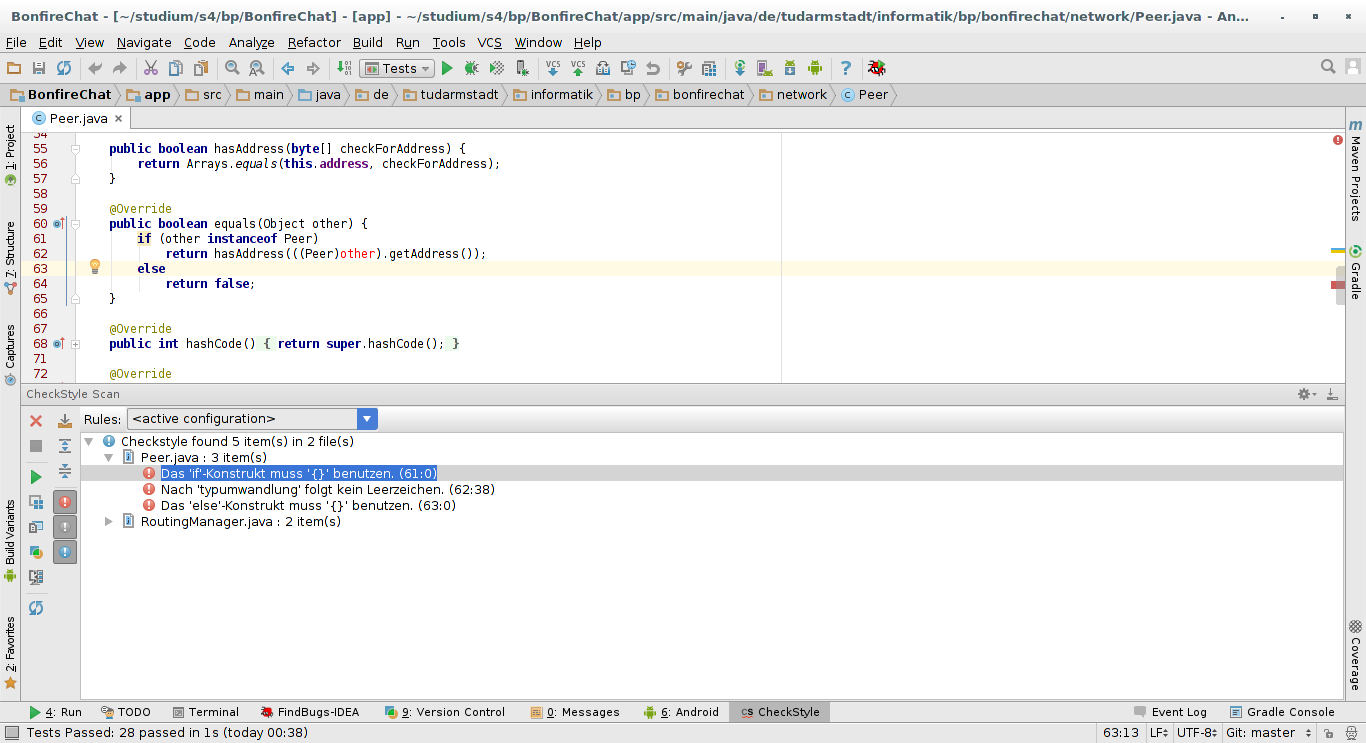
\includegraphics[width=17.5cm]{belege/checkstyle/checkstyle-idea-screenshot.png}


\clearpage
\subsection{Android Lint}

Zusätzlich haben wir das von Google entwickelte und empfohlene ``Android Lint''
genutzt. Dieses Tool gibt Empfehlungen zur Einhaltung der Android-Programmierrichtlinien.

Dadurch verbessert sich einerseits die Wartbarkeit, denn durch das Befolgen der im Android-Umfeld üblichen
 Konventionen und die Verwendung von allgemein bekannten und anerkannten Entwurfsmustern, ist der Code zukünftigen
Entwicklern leichter verständlich.
Andererseits enthalten die Reports Empfehlungen zur Verbesserung der Performance, Usability, Accessibility und Korrektheit.

Im folgenden Abschnitt befindet sich ein Report, der erstellt wurde,
als wir begonnen haben, ``Android Lint'' einzusetzen. Dann wurden initial alle
Warnungen und Empfehlungen abgearbeitet (Commit XXXXXXXXXXXXX TODO).
Die Warnungen und Empfehlungen werden direkt in der von uns verwendeten
Entwicklungsumgebung Android Studio angezeigt, sodass diese anschließend während
der Programmierung direkt umgesetzt werden konnten. Daher ist der zweite Report,
der zum Abschluss des Projekts erstellt wurde, leer.


\includepdf[pages=1,offset=-0.8cm 0,scale=.8,pagecommand=\subsubsection{Initialer ``Android Lint''-Report}]{anhang/partials/lint-results-1.pdf}
\includepdf[pages=2-,offset=-0.8cm 0,scale=.8,pagecommand={}]{anhang/partials/lint-results-1.pdf}

\includepdf[pages=1,offset=-0.8cm 0,scale=.8,pagecommand=\subsubsection{Finaler ``Android Lint''-Report}]{anhang/partials/lint-results-2.pdf}
%\includepdf[pages=2-,scale=.8,pagecommand={}]{anhang/partials/lint-results-2.pdf}


\clearpage
\subsection{FindBugs}

Um häufig auftretende Fehler zu vermeiden, haben wir FindBugs verwendet.

Im folgenden Abschnitt befindet sich ein Report, der erstellt wurde, als wir mit der Verwendung von ``FindBugs'' begonnen aben. Anschließend wurden alle Fehler und Warnungen in Commit XXXXXXXX TODO behoben. Da wir das Plugin FindBugs-IDEA direkt in unsere Entwicklungsumgebung integriert haben und Fehler so direkt markiert wurden, konnten Fehler ab dann direkt bei der Entwicklung vermieden werden und der zweite, am Ende des Projektes erstellte, Report ist leer.


\includepdf[pages=1,offset=-0.8cm 0,scale=.8,pagecommand=\subsubsection{Initialer ``FindBugs''-Report}]{anhang/partials/findbugs-1.pdf}
\includepdf[pages=2-,offset=-0.8cm 0,scale=.8,pagecommand={}]{anhang/partials/findbugs-1.pdf}

\includepdf[pages=1,offset=-0.8cm 0,scale=.8,pagecommand=\subsubsection{Finaler ``FindBugs''-Report}]{anhang/partials/findbugs-2.pdf}
\includepdf[pages=2-,offset=-0.8cm 0,scale=.8,pagecommand={}]{anhang/partials/findbugs-2.pdf}


\clearpage

% ---------------------------------------------------------------------------
% Code Reviews (Einleitung)

\section{Code Reviews}

Zur Sicherstellung der Wartbarkeit durch hohe Code-Qualität wurde bei jedem
Sprint-Treffen mit dem Auftraggeber ein Code Review durchgeführt.

% ---------------------------------------------------------------------------
% Code Reviews: Checkliste

\subsection{Checkliste}


\begin{enumerate}[ 1.]
  \item Ist die Funktionalität korrekt?
  \item Sind die Klassen, Funktionen und Variablen angemessen benannt?
  \item Wurde die Klassenstruktur gut entworfen und erfüllt sie alle Anforderungen, oder sind Verbesserungen nötig?
  \item Gibt es Klassen, die aufgrund neuer Implementierungen überflüssig geworden sind?
  \item Gibt es unnötig überladene Funktionen oder Konstruktoren?
  \item Wurde die Datenbankstruktur gut entworfen?
  \item Enthält das Codeteil Funktionen, die wiederverwendet werden können? Sind diese in einer Helper-Klasse untergebracht?
  \item Wurden existierende Helper-Funktionen benutzt? Ist keine doppelte Funktionalität implementiert?
  \item Werden alle Eingabeparameter validiert?
  \item Wie beeinflusst die Funktionalität die Performance der App - Stromverbrauch, Rechenzeit und Speicherbedarf?
  \item Ist es unbedingt nötig, den Code in einem UI-Thread laufen zu lassen oder würde ein Background-Thread ausreichen?
  \item Werden alle möglichen Fehlschläge behandelt?
  \item Findet eine ``Graceful Degradation'' statt?
  \item Werden die Best Practices zur Appentwicklung, laut Android Lint, befolgt?
  \item Welche Teile können parallel ausgeführt werden?
  \item Sind die Operationen, bei denen Threadsicherheit benötigt wird, threadsicher?
  \item Ist das Layout passend für alle Bildschirmdimensionen?
  \item Haben alle Methoden und Felder die richtigen Zugriffsmodifier?
\end{enumerate}


% ---------------------------------------------------------------------------
% Code Reviews: Ergebnisse
\input{anhang/partials/codereviews.tex}


\clearpage
\section{Dokumentation}

Um die Wartung der Anwendung in Zukunft zu erleichtern, wurden die technischen Grundlagen
sowie alle wichtigen Designentscheidungen in einem Dokument festgehalten.

\input{anhang/partials/dokumentation.tex}



% ---------------------------------------------------------------------------
% Automatisierte Tests: (Einleitung)

\clearpage
\section{Automatisierte Tests}

Es wurden JUnit-Tests für die automatisiert testbaren Codeteile durchgeführt.
Im folgenden findet sich zunächst eine Liste aller Tests sowie der Testergebnisse,
außerdem das Ergebnis der Test-Coverage-Analyse, aufgeschlüsselt nach Packages.
\\\\
Wie bereits im QS-Dokument beschrieben, war ein Testen des UI- und Netzwerkcodes
(Packages bonfirechat.network und bonfirechat.ui)
mit dem JUnit-Framework nicht möglich, da die Android-Klassenbibliothek dort nicht
zur Verfügung steht. Das gleiche gilt für die Datenbankklasse, da diese von einer
Android-internen Klasse erbt. Daher konnte auch die Klasse bonfire.data.BonfireData
nicht mit automatisierten Tests versehen werden.
\\\\
Zusammenfassend gilt, dass wir automatisierte Tests für alle Methoden geschrieben haben,
die
\begin{itemize}
\item keine Klassen der Android-Klassenbibliothek verwenden,
\item Klassen der Android-Klassenbibliothek nur als Parameter übergeben bekommen,
sodass wir stattdessen mit Mockito erstellte Mock-Objekte übergeben können, oder
\item mit vertretbarem Aufwand angepasst werden konnten, sodass der vorhergehende Punkt zutrifft.
\end{itemize}

% ---------------------------------------------------------------------------
% Automatisierte Tests: Javadoc-Testplan

\includepdf[pages=1,scale=.8,pagecommand=\subsection{Testplan}]{anhang/partials/javadoc.pdf}
\includepdf[pages=2-,scale=.8,pagecommand={}]{anhang/partials/javadoc.pdf}

% ---------------------------------------------------------------------------
% Automatisierte Tests: Ergebnisse

\includepdf[pages=1,offset=-0.8cm 0,scale=.8,pagecommand=\subsection{Ergebnisse}]{anhang/partials/junit.pdf}
\includepdf[pages=2-,offset=-0.8cm 0,scale=.8,pagecommand={}]{anhang/partials/junit.pdf}


% ---------------------------------------------------------------------------
% Automatisierte Tests: Test Coverage

\includepdf[pages=-,offset=-0.8cm 0,scale=.8,pagecommand=\subsection{Test Coverage}]{anhang/partials/coverage.pdf}



\clearpage

\section{Manuelle Tests der Benutzeroberfläche}

Da uns der Aufwand für die Nutzung eines Instrumented-Test-Frameworks
für das recht einfache User Interface der App unverhältnismäßig
erscheint, werden manuelle Tests anhand der folgenden Testpläne
vorgenommen.

\subsection{Testplan}

Dieser Abschnitt beschreibt einen Testplan für manuelles Testen der
drahtlosen Übertragung sowie des Routing-Algorithmus.\\\\

% ----------------------------------------------------------------------

\subsubsection{N-i: Definitionen}\label{i-definitionen}

\paragraph{Allgemeine Ausgangskonfiguration der
Knoten:}\label{allgemeine-ausgangskonfiguration-der-knoten}

Ein Knoten ist, soweit nicht näher beschrieben, ein Android-Gerät, auf
dem die aktuellste Version der App eingerichtet und die initiale
Einrichtung (Eingabe eines Nicknames, dadurch Registrierung des Gerätes
mit Nickname, GCM-ID und PublicKey am Server) abgeschlossen ist.


% ----------------------------------------------------------------------
% II

\clearpage
\subsubsection{N-ii: Testfälle für die allgemeine
Übertragung}\label{ii-testfuxe4lle-fuxfcr-die-allgemeine-uxfcbertragung}

\paragraph{N-ii-1. Test der direkten Übertragung via Flooding /
Bluetooth}\label{test-der-direkten-uxfcbertragung-via-flooding-bluetooth}

\begin{longtable}{p{8cm}p{8.5cm}}
\toprule
Benutzerinteraktion & erwartetes Verhalten der App\tabularnewline
\midrule
\endhead
Auf zwei Knoten A und B, die sich in direkter Bluetooth-Reichweite
befinden, wird zunächst die Ausgangskonfiguration hergestellt,
anschließend werden in den Einstellungen alle Übertragungsverfahren
außer Bluetooth deaktiviert. Die Kontaktdaten von A werden an B
gesendet. Auf B wird eine neue Unterhaltung mit A gestartet. Auf B wird
eine Nachricht an A eingegeben und abgesendet. & B sendet die Nachricht
an alle per Bluetooth sichtbaren Geräte, insbesondere an A. Auf A wird
die Nachricht empfangen und als per Bluetooth empfangen dargestellt. A
sendet ein ACK an B, dieses wird auf B durch ein Häkchen an der
Nachricht sichtbar. Weiterhin erscheint ein Bluetooth-Icon an der
Nachricht, da die Nachricht per Bluetooth zugestellt wurde. Im Dashboard
ist erkennbar, dass die Nachricht mit Routingmodus Flooding (0x01)
versendet wurde, das ACK mit Routingmodus DSR (0x02).\tabularnewline
\bottomrule
\end{longtable}

\paragraph{N-ii-2. Test der direkten Übertragung via DSR /
Bluetooth}\label{test-der-direkten-uxfcbertragung-via-dsr-bluetooth}

\begin{longtable}{p{8cm}p{8.5cm}}
\toprule
Benutzerinteraktion & erwartetes Verhalten der App\tabularnewline
\midrule
\endhead
Nach der erfolgreichen Durchführung von Test 1 wird eine weitere
Nachricht von B an A gesendet, sowie eine Nachricht von A an B. & Nach
Test 1 ist den Geräten A und B der schnellste Pfad zum jeweils anderen
Gerät bekannt. Daher sendet B die Nachricht nicht per Routingmodus
Flooding (0x01), sondern per Dynamic Source Routing (0x02), also unter
der Angabe der gewünschten Übertragungspfades. Daher wird die Nachricht
nur an Gerät A gesendet. Darüber hinaus identisch zu Test
1.\tabularnewline
\bottomrule
\end{longtable}

\paragraph{N-ii-3. Test der direkten Übertragung via Server / Google Cloud
Messaging}\label{test-der-direkten-uxfcbertragung-via-server-google-cloud-messaging}

\begin{longtable}{p{8cm}p{8.5cm}}
\toprule
Benutzerinteraktion & erwartetes Verhalten der App\tabularnewline
\midrule
\endhead
Auf zwei Knoten A und B, die eine funktionierende Internetverbindung
haben, wird zunächst die Ausgangskonfiguration hergestellt, anschließend
werden in den Einstellungen alle Übertragungsverfahren außer ``mobile
Daten / Wifi'' (Übertragung per Cloud) deaktiviert. Die Kontaktdaten von
A werden an B gesendet. Auf B wird eine neue Unterhaltung mit A
gestartet. Auf B wird eine Nachricht an A eingegeben und abgesendet. & B
sendet die Nachricht per HTTP an den Server, welcher sie per GCM an
Gerät A weiterleitet. Auf A wird die Nachricht empfangen und als per
Cloud empfangen dargestellt. A sendet ein ACK an B, dieses wird auf B
durch ein Häkchen an der Nachricht sichtbar. Weiterhin erscheint ein
Cloud-Icon an der Nachricht, da die Nachricht per Cloud zugestellt
wurde. Im Dashboard ist erkennbar, dass die Nachricht mit Routingmodus
Flooding (0x01) versendet wurde, das ACK mit Routingmodus DSR
(0x02).\tabularnewline
\bottomrule
\end{longtable}


% ----------------------------------------------------------------------
% III

\clearpage
\subsubsection{N-iii: Testfälle für Wegfindung per Flooding und einfaches
Routing}\label{iii-testfuxe4lle-fuxfcr-wegfindung-per-flooding-und-einfaches-routing}

In diesen Tests werden folgende Teile des Routing getestet: * Finden des
schnellsten Pfades: Flooding an alle Knoten sowie ACK auf dem Pfad, auf
dem die Nachricht den Empfänger zuerst erreicht (= schnellster Pfad) *
Speichern des schnellsten Pfades zu einem Empfänger * Verwenden des
gespeicherten schnellsten Pfades für künftige Nachrichten

\paragraph{N-iii-1. Bluetooth-Wegfindung - Flooding mit drei
Knoten}\label{bluetooth-wegfindung---flooding-mit-drei-knoten}

\begin{longtable}{p{8cm}p{8.5cm}}
\toprule
Benutzerinteraktion & erwartetes Verhalten der App\tabularnewline
\midrule
\endhead
Auf drei Knoten A, B und C werden alle Übertragungsverfahren außer
Bluetooth deaktiviert. Die Kontaktdetails von C werden an A gesendet.
Die Knoten werden räumlich so angeordnet, dass eine Bluetoothverbindung
zwischen A und B sowie zwischen B und C möglich ist, nicht jedoch
zwischen A und C. Auf A wird eine Unterhaltung mit C begonnen und eine
Nachricht an C gesendet. & Nachricht u. ACK kommen an,
etc.\tabularnewline
\bottomrule
\end{longtable}

\paragraph{N-iii-2. Bluetooth-Wegfindung zum nächsten Knoten mit
Internetverbindung}\label{bluetooth-wegfindung-zum-nuxe4chsten-knoten-mit-internetverbindung}

\begin{longtable}{p{8cm}p{8.5cm}}
\toprule
Benutzerinteraktion & erwartetes Verhalten der App\tabularnewline
\midrule
\endhead
Knoten A, B und C werden wie in Testfall III.1 vorbereitet. Auf Knoten C
wird zusätzlich die Übertragung per Cloud aktiviert. Auf einem weiteren
Knoten D wird nur die Übertragung per Cloud aktiviert. Es wird
sichergestellt, dass C und D mit dem Internet verbunden sind. Die
Kontaktdetails von D werden an A gesendet. A beginnt eine Unterhaltung
mit D und sendet die Nachricht ``alpha'' an D. Nach Erhalt der Nachricht
``alpha'' sendet A eine weitere Nachricht ``beta''. & Die Nachricht
``alpha'' kommt per Flooding über B, C und Server bei D an, ACK ``für
alpha'' geht auf direktem Pfad (D-Server-C-B-A) per DSR zurück an A. Die
Nachricht ``beta'' wird auf direktem Pfad (A-B-C-Server-D) per DSR an D
gesendet, ACK ``für beta'' wie ACK ``für alpha''. Die empfangenen und
weitergeleiteten Nachrichten und ihre Pfade sind entsprechend im
Dashboard ersichtlich.\tabularnewline
\bottomrule
\end{longtable}

\paragraph{N-iii-3.}\label{section}

TODO Test beschreiben




% ------------------------------------------------------------------------
% IV

\clearpage
\subsubsection{N-iv: Testfälle für sich verändernde
Routen}\label{iv-testfuxe4lle-fuxfcr-sich-veruxe4ndernde-routen}

In diesen Tests wird überprüft, ob der Routingalgorithmus bei
ausfallenden Pfaden korrekt reagiert.

\paragraph{\texorpdfstring{N-iv-1. ``Abreißende''
Bluetooth-Verbindung}{N-iv-1. Abreißende Bluetooth-Verbindung}}\label{abreiuxdfende-bluetooth-verbindung}

\begin{longtable}{p{8cm}p{8.5cm}}
\toprule
Benutzerinteraktion & erwartetes Verhalten der App\tabularnewline
\midrule
\endhead
Auf drei Knoten A wird nur Bluetooth aktiviert, auf B wird GCM und
Bluetooth aktiviert. Von A wird eine Nachricht ``alpha'' an B gesendet.
Nachdem diese zugestellt und acknowledged wurde, wird eine weitere
Nachricht ``beta'' von A and B gesendet. Danach wird A räumlich so weit
vom B entfernt, dass keine Bluetooth-Übertragung mehr möglich ist.
Weiterhin wird auf A die Übertragung per GCM aktiviert. Anschließend
wird eine weitere Nachricht ``gamma'' von A and B gesendet. & Die
Nachricht ``alpha'' wird per Flooding gesendet, B sendet per DSR ein ACK
``für alpha'' zurück. Danach hat A den Pfad zu B gespeichert und die
Nachricht ``beta'' wird direkt per DSR an B gesendet. Die Nachricht
``gamma'' wird auch versucht per DSR direkt via Bluetooth an B zu
senden. Da dies fehlschlägt, wird beim Retry nach 20 Sekunden versucht,
``gamma'' per Flooding zuzustellen. Dies erfolgt dann über GCM. Das ACK
``für gamma'' von B an A erfolgt dann wiederum per DSR.\tabularnewline
\bottomrule
\end{longtable}



% ------------------------------------------------------------------------
% V

\clearpage
\subsubsection{N-v: Testfälle für Störeinflüsse im
Netzwerk}\label{v-testfuxe4lle-fuxfcr-stuxf6reinfluxfcsse-im-netzwerk}

Hier soll überprüft werden, wie sich die App bei äußeren Störeinflüssen
auf Netzwerkebene, also zum Beispiel während einer während der
Datenübertragung abreißenden Verbindung, verhält. Es soll sichergestellt
sein, dass stets angemessen reagiert wird und sowohl die App nicht
abstürzt als auch der Benutzer sinnvolle Fehlermeldungen erhält.

Da dies teilweise sporadische Fehler sind, welche sich schwer
reproduzieren lassen, ist die Aussagekraft der folgenden Tests leider
nur bedingt gegeben.

\paragraph{\texorpdfstring{N-v-1. ``Socket wird unerwartet während der
Verbindung
geschlossen''}{N-v-1. Socket wird unerwartet während der Verbindung geschlossen}}\label{socket-wird-unerwartet-wuxe4hrend-der-verbindung-geschlossen}

\begin{longtable}{p{8cm}p{8.5cm}}
\toprule
Benutzerinteraktion & erwartetes Verhalten der App\tabularnewline
\midrule
\endhead
\bottomrule
\end{longtable}

\paragraph{N-v-2. Benutzer schaltet Bluetooth im Telefon
aus}\label{benutzer-schaltet-bluetooth-im-telefon-aus}

\begin{longtable}{p{8cm}p{8.5cm}}
\toprule
Benutzerinteraktion & erwartetes Verhalten der App\tabularnewline
\midrule
\endhead
\bottomrule
\end{longtable}


\input{anhang/partials/manuelle-tests-ui-reports.tex}


\clearpage
\section{Manueller Test für Routing und Datenübertragungs-Protokolle}
\subsection{Testplan}

Dieser Abschnitt beschreibt einen Testplan für manuelles Testen der
drahtlosen Übertragung sowie des Routing-Algorithmus.\\\\

% ----------------------------------------------------------------------

\subsubsection{N-i: Definitionen}\label{i-definitionen}

\paragraph{Allgemeine Ausgangskonfiguration der
Knoten:}\label{allgemeine-ausgangskonfiguration-der-knoten}

Ein Knoten ist, soweit nicht näher beschrieben, ein Android-Gerät, auf
dem die aktuellste Version der App eingerichtet und die initiale
Einrichtung (Eingabe eines Nicknames, dadurch Registrierung des Gerätes
mit Nickname, GCM-ID und PublicKey am Server) abgeschlossen ist.


% ----------------------------------------------------------------------
% II

\clearpage
\subsubsection{N-ii: Testfälle für die allgemeine
Übertragung}\label{ii-testfuxe4lle-fuxfcr-die-allgemeine-uxfcbertragung}

\paragraph{N-ii-1. Test der direkten Übertragung via Flooding /
Bluetooth}\label{test-der-direkten-uxfcbertragung-via-flooding-bluetooth}

\begin{longtable}{p{8cm}p{8.5cm}}
\toprule
Benutzerinteraktion & erwartetes Verhalten der App\tabularnewline
\midrule
\endhead
Auf zwei Knoten A und B, die sich in direkter Bluetooth-Reichweite
befinden, wird zunächst die Ausgangskonfiguration hergestellt,
anschließend werden in den Einstellungen alle Übertragungsverfahren
außer Bluetooth deaktiviert. Die Kontaktdaten von A werden an B
gesendet. Auf B wird eine neue Unterhaltung mit A gestartet. Auf B wird
eine Nachricht an A eingegeben und abgesendet. & B sendet die Nachricht
an alle per Bluetooth sichtbaren Geräte, insbesondere an A. Auf A wird
die Nachricht empfangen und als per Bluetooth empfangen dargestellt. A
sendet ein ACK an B, dieses wird auf B durch ein Häkchen an der
Nachricht sichtbar. Weiterhin erscheint ein Bluetooth-Icon an der
Nachricht, da die Nachricht per Bluetooth zugestellt wurde. Im Dashboard
ist erkennbar, dass die Nachricht mit Routingmodus Flooding (0x01)
versendet wurde, das ACK mit Routingmodus DSR (0x02).\tabularnewline
\bottomrule
\end{longtable}

\paragraph{N-ii-2. Test der direkten Übertragung via DSR /
Bluetooth}\label{test-der-direkten-uxfcbertragung-via-dsr-bluetooth}

\begin{longtable}{p{8cm}p{8.5cm}}
\toprule
Benutzerinteraktion & erwartetes Verhalten der App\tabularnewline
\midrule
\endhead
Nach der erfolgreichen Durchführung von Test 1 wird eine weitere
Nachricht von B an A gesendet, sowie eine Nachricht von A an B. & Nach
Test 1 ist den Geräten A und B der schnellste Pfad zum jeweils anderen
Gerät bekannt. Daher sendet B die Nachricht nicht per Routingmodus
Flooding (0x01), sondern per Dynamic Source Routing (0x02), also unter
der Angabe der gewünschten Übertragungspfades. Daher wird die Nachricht
nur an Gerät A gesendet. Darüber hinaus identisch zu Test
1.\tabularnewline
\bottomrule
\end{longtable}

\paragraph{N-ii-3. Test der direkten Übertragung via Server / Google Cloud
Messaging}\label{test-der-direkten-uxfcbertragung-via-server-google-cloud-messaging}

\begin{longtable}{p{8cm}p{8.5cm}}
\toprule
Benutzerinteraktion & erwartetes Verhalten der App\tabularnewline
\midrule
\endhead
Auf zwei Knoten A und B, die eine funktionierende Internetverbindung
haben, wird zunächst die Ausgangskonfiguration hergestellt, anschließend
werden in den Einstellungen alle Übertragungsverfahren außer ``mobile
Daten / Wifi'' (Übertragung per Cloud) deaktiviert. Die Kontaktdaten von
A werden an B gesendet. Auf B wird eine neue Unterhaltung mit A
gestartet. Auf B wird eine Nachricht an A eingegeben und abgesendet. & B
sendet die Nachricht per HTTP an den Server, welcher sie per GCM an
Gerät A weiterleitet. Auf A wird die Nachricht empfangen und als per
Cloud empfangen dargestellt. A sendet ein ACK an B, dieses wird auf B
durch ein Häkchen an der Nachricht sichtbar. Weiterhin erscheint ein
Cloud-Icon an der Nachricht, da die Nachricht per Cloud zugestellt
wurde. Im Dashboard ist erkennbar, dass die Nachricht mit Routingmodus
Flooding (0x01) versendet wurde, das ACK mit Routingmodus DSR
(0x02).\tabularnewline
\bottomrule
\end{longtable}


% ----------------------------------------------------------------------
% III

\clearpage
\subsubsection{N-iii: Testfälle für Wegfindung per Flooding und einfaches
Routing}\label{iii-testfuxe4lle-fuxfcr-wegfindung-per-flooding-und-einfaches-routing}

In diesen Tests werden folgende Teile des Routing getestet: * Finden des
schnellsten Pfades: Flooding an alle Knoten sowie ACK auf dem Pfad, auf
dem die Nachricht den Empfänger zuerst erreicht (= schnellster Pfad) *
Speichern des schnellsten Pfades zu einem Empfänger * Verwenden des
gespeicherten schnellsten Pfades für künftige Nachrichten

\paragraph{N-iii-1. Bluetooth-Wegfindung - Flooding mit drei
Knoten}\label{bluetooth-wegfindung---flooding-mit-drei-knoten}

\begin{longtable}{p{8cm}p{8.5cm}}
\toprule
Benutzerinteraktion & erwartetes Verhalten der App\tabularnewline
\midrule
\endhead
Auf drei Knoten A, B und C werden alle Übertragungsverfahren außer
Bluetooth deaktiviert. Die Kontaktdetails von C werden an A gesendet.
Die Knoten werden räumlich so angeordnet, dass eine Bluetoothverbindung
zwischen A und B sowie zwischen B und C möglich ist, nicht jedoch
zwischen A und C. Auf A wird eine Unterhaltung mit C begonnen und eine
Nachricht an C gesendet. & Nachricht u. ACK kommen an,
etc.\tabularnewline
\bottomrule
\end{longtable}

\paragraph{N-iii-2. Bluetooth-Wegfindung zum nächsten Knoten mit
Internetverbindung}\label{bluetooth-wegfindung-zum-nuxe4chsten-knoten-mit-internetverbindung}

\begin{longtable}{p{8cm}p{8.5cm}}
\toprule
Benutzerinteraktion & erwartetes Verhalten der App\tabularnewline
\midrule
\endhead
Knoten A, B und C werden wie in Testfall III.1 vorbereitet. Auf Knoten C
wird zusätzlich die Übertragung per Cloud aktiviert. Auf einem weiteren
Knoten D wird nur die Übertragung per Cloud aktiviert. Es wird
sichergestellt, dass C und D mit dem Internet verbunden sind. Die
Kontaktdetails von D werden an A gesendet. A beginnt eine Unterhaltung
mit D und sendet die Nachricht ``alpha'' an D. Nach Erhalt der Nachricht
``alpha'' sendet A eine weitere Nachricht ``beta''. & Die Nachricht
``alpha'' kommt per Flooding über B, C und Server bei D an, ACK ``für
alpha'' geht auf direktem Pfad (D-Server-C-B-A) per DSR zurück an A. Die
Nachricht ``beta'' wird auf direktem Pfad (A-B-C-Server-D) per DSR an D
gesendet, ACK ``für beta'' wie ACK ``für alpha''. Die empfangenen und
weitergeleiteten Nachrichten und ihre Pfade sind entsprechend im
Dashboard ersichtlich.\tabularnewline
\bottomrule
\end{longtable}

\paragraph{N-iii-3.}\label{section}

TODO Test beschreiben




% ------------------------------------------------------------------------
% IV

\clearpage
\subsubsection{N-iv: Testfälle für sich verändernde
Routen}\label{iv-testfuxe4lle-fuxfcr-sich-veruxe4ndernde-routen}

In diesen Tests wird überprüft, ob der Routingalgorithmus bei
ausfallenden Pfaden korrekt reagiert.

\paragraph{\texorpdfstring{N-iv-1. ``Abreißende''
Bluetooth-Verbindung}{N-iv-1. Abreißende Bluetooth-Verbindung}}\label{abreiuxdfende-bluetooth-verbindung}

\begin{longtable}{p{8cm}p{8.5cm}}
\toprule
Benutzerinteraktion & erwartetes Verhalten der App\tabularnewline
\midrule
\endhead
Auf drei Knoten A wird nur Bluetooth aktiviert, auf B wird GCM und
Bluetooth aktiviert. Von A wird eine Nachricht ``alpha'' an B gesendet.
Nachdem diese zugestellt und acknowledged wurde, wird eine weitere
Nachricht ``beta'' von A and B gesendet. Danach wird A räumlich so weit
vom B entfernt, dass keine Bluetooth-Übertragung mehr möglich ist.
Weiterhin wird auf A die Übertragung per GCM aktiviert. Anschließend
wird eine weitere Nachricht ``gamma'' von A and B gesendet. & Die
Nachricht ``alpha'' wird per Flooding gesendet, B sendet per DSR ein ACK
``für alpha'' zurück. Danach hat A den Pfad zu B gespeichert und die
Nachricht ``beta'' wird direkt per DSR an B gesendet. Die Nachricht
``gamma'' wird auch versucht per DSR direkt via Bluetooth an B zu
senden. Da dies fehlschlägt, wird beim Retry nach 20 Sekunden versucht,
``gamma'' per Flooding zuzustellen. Dies erfolgt dann über GCM. Das ACK
``für gamma'' von B an A erfolgt dann wiederum per DSR.\tabularnewline
\bottomrule
\end{longtable}



% ------------------------------------------------------------------------
% V

\clearpage
\subsubsection{N-v: Testfälle für Störeinflüsse im
Netzwerk}\label{v-testfuxe4lle-fuxfcr-stuxf6reinfluxfcsse-im-netzwerk}

Hier soll überprüft werden, wie sich die App bei äußeren Störeinflüssen
auf Netzwerkebene, also zum Beispiel während einer während der
Datenübertragung abreißenden Verbindung, verhält. Es soll sichergestellt
sein, dass stets angemessen reagiert wird und sowohl die App nicht
abstürzt als auch der Benutzer sinnvolle Fehlermeldungen erhält.

Da dies teilweise sporadische Fehler sind, welche sich schwer
reproduzieren lassen, ist die Aussagekraft der folgenden Tests leider
nur bedingt gegeben.

\paragraph{\texorpdfstring{N-v-1. ``Socket wird unerwartet während der
Verbindung
geschlossen''}{N-v-1. Socket wird unerwartet während der Verbindung geschlossen}}\label{socket-wird-unerwartet-wuxe4hrend-der-verbindung-geschlossen}

\begin{longtable}{p{8cm}p{8.5cm}}
\toprule
Benutzerinteraktion & erwartetes Verhalten der App\tabularnewline
\midrule
\endhead
\bottomrule
\end{longtable}

\paragraph{N-v-2. Benutzer schaltet Bluetooth im Telefon
aus}\label{benutzer-schaltet-bluetooth-im-telefon-aus}

\begin{longtable}{p{8cm}p{8.5cm}}
\toprule
Benutzerinteraktion & erwartetes Verhalten der App\tabularnewline
\midrule
\endhead
\bottomrule
\end{longtable}


\subsection{Durchführung}
\subsubsection{Durchführung des manuellen Netzwerk-Testplans vom 30.08.2015}

\subsubsection{Durchgeführt von: Matthias Hofmann}

\subsubsection{Änderungen vorgenommen in Commit: keine Änderungen nötig}

\subsubsection{N-i: Allgemeine Informationen zu den Testergebnissen}

\paragraph{N-i.1. Packet Attribute im Dashboard}
Die Spaltenfunktionalität im Dashboard ist der Reihe nach aufgelistet:
-Gerät, das die Informations ans Dashboard sendet
-Ereignis, das den Informationsautsch auslöst
-Uhrzeit des Ereignis
-Verwendetes Übertragungsprotokoll
-Adresse des Empfängers(Falls Ereignis = "SEND")
-Packetdetails

In der sechsten Spalte im Dashboard werden Details der Übertragung dargestellt. 
Dabei ist die eindeutige ID der Nachricht das zweite Attribut vom Packet.
Desweiteren steht "routing=1" für senden via Flooding und "routing=2" für senden via DRS-Adaption.

\paragraph{N-i.2. Zeiten der Nachrichten im Dashboard}
Die angegebenen Zeiten der Ereignisse im Dashboard wirken auf den ersten Blick unwahrscheinlich. 
Zum Beispeiel wird in Test II)1. ein Acknowledgement zuersst empfangen, bevor es gesendet wurde.
Dies liegt daran, dass die Übertragungn des Ackknowledgements per Bluetooth stattgefunden hat und das Gerät, 
dass diese Empfangen hat, eine schnellere Verbindung zum Dashboard server hatte. 
Somit wurde das Dashboard zuerst über das Ankommen des ACK informiert und dann erst über das Versenden.


\subsubsection{N-ii: Testfälle für die allgemeine Übertragung}

\paragraph{N-i.1 Test der direkten Übertragung via Flooding / Bluetooth}
Beschreibung des Ergebnisses in Test II)1.

\section{Großtests}
\subsection{Testplan}
% Add Testplan here \input{}

\clearpage\subsection{Testbericht}\label{testbericht}

Die Handys wurden mit Buchstaben benannt und im Raum C205 verteilt.

\clearpage\subsection{Ergebnisse Test 1:}\label{ergebnisse-test-1}

Wir haben auf 117 Nachrichten 11 erfolgreiche Fälle und 106 Errors.
\\\\
\textbf{Folgende Beispiele veranschaulichen Nachrichten, die beim
Empfänger angekommen sind:}
\\\\
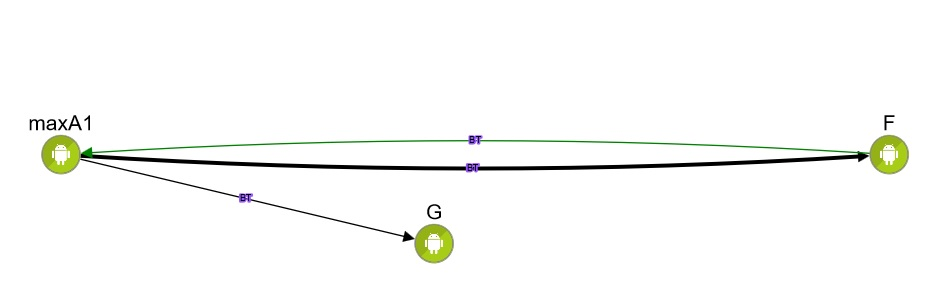
\includegraphics[width=1.0\textwidth]{belege/grosstests/Bilder/Erfolg4.jpg}\\
1. A sendet eine Nachricht an F. A sendet die Nachricht an G und F los, da A nur den
Bluetooth Namen der Handys kennt, und so nicht weiß, dass F sich in
Reichweite befindet. F sendet ein Acknowledgement zurück, während G die
Nachricht nicht weiterleiten kann.\\
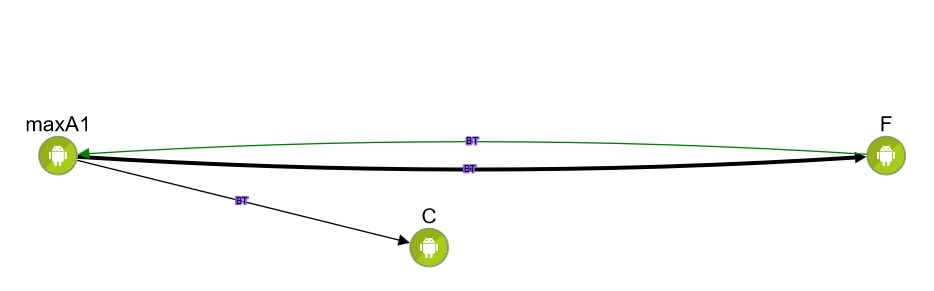
\includegraphics[width=1.0\textwidth]{belege/grosstests/Bilder/Erfolg3.jpg}\\
2. Gleiches Scenario wie in 2, nur diesmal mit C statt G.\\
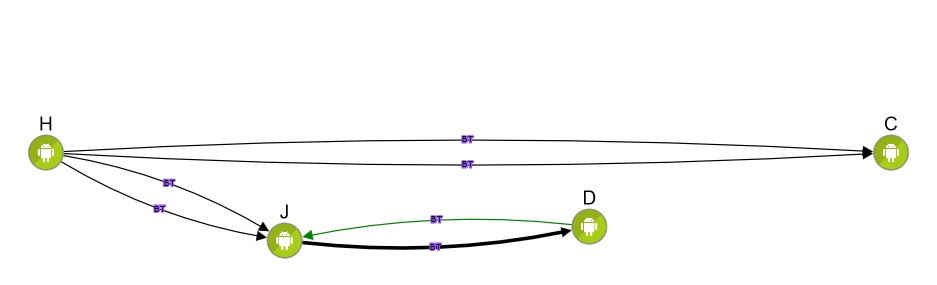
\includegraphics[width=1.0\textwidth]{belege/grosstests/Bilder/Erfolg2.jpg}\\ 3. H sendet eine
Nachricht an D. Es befinden sich J und C in Reichweite. C leitet die
Nachricht nicht weiter. J hat jedoch eine Verbindung zu D. D sendet ein
Acknowledgement über den Pfad, über den er die Nachricht empfangen hat
zurück.\\ 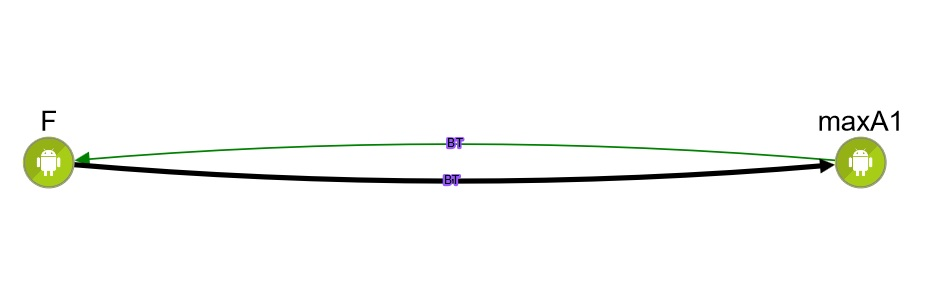
\includegraphics[width=1.0\textwidth]{belege/grosstests/Bilder/Erfolg1.jpg} \\4. Eine
Erfolgreich übertragene Nachricht zwischen 2 benachbarten Handys mit
Acknowledgement.
\\\\
\textbf{Folgende Beispiele veranschaulichen Nachrichten, die nicht beim
Empfänger angekommen sind:}\\
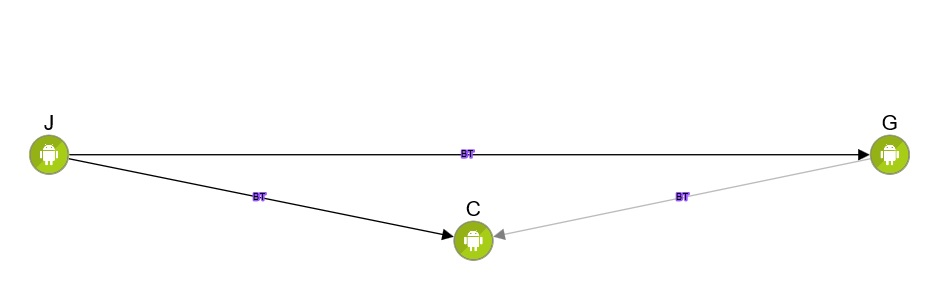
\includegraphics[width=1.0\textwidth]{belege/grosstests/Bilder/Miserfolg6.jpg}\\ 1. J versucht
eine Nachricht zu schicken. Es befinden sich jedoch nur die Handys G und
C in Reichweite. G kann daraufhin nur Verbindung mit C herstellen, das
jedoch die Nachricht bereits kennt.\\
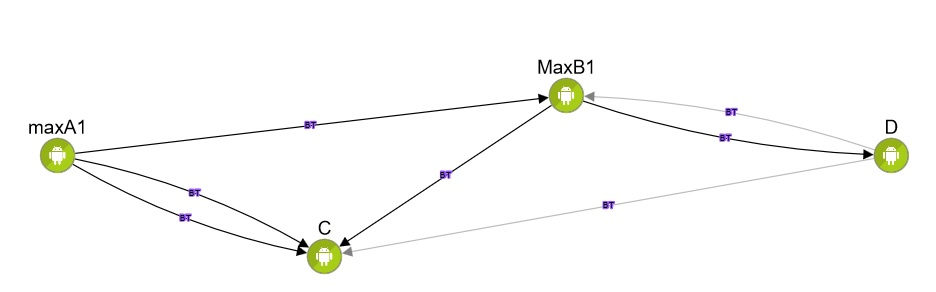
\includegraphics[width=1.0\textwidth]{belege/grosstests/Bilder/Miserfolg5.jpg}\\ 2. A versucht
eine Nachricht zu schicken. Es befinden sich jedoch nur die Handys B und
C in Reichweite. B kann die Nachricht nun noch an D weiterleiten. Dort
bleibt sie jedoch hängen, da D nur noch eine Verbindung zu C findet, das
die Nachricht bereits kennt. A versucht daraufhin in einem Retry die
Nachricht erneut zu schicken, findet aber nun nur noch C.\\
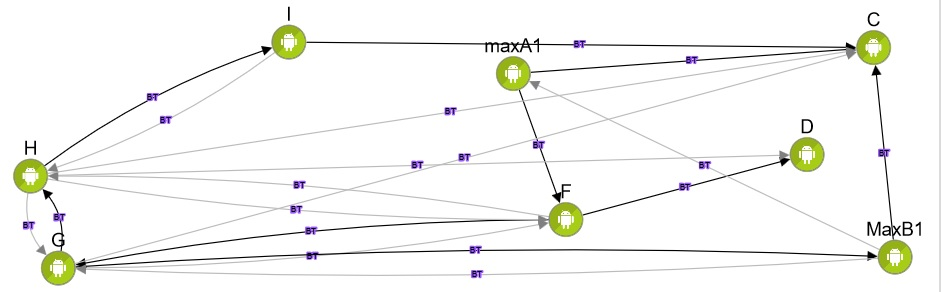
\includegraphics[width=1.0\textwidth]{belege/grosstests/Bilder/Miserfolg4.jpg}\\ 3. An diesem
Beispiel erkennt man, dass alle Handys nah zueinander lagen. Die
Nachricht wird von A verschickt. Sie durchläuft 7 der 9 anderen Handys.\\
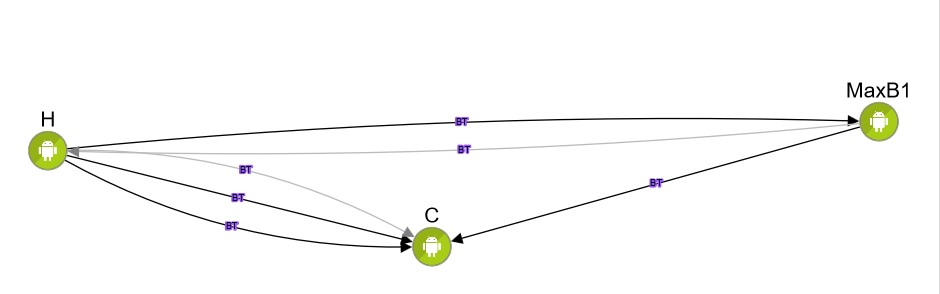
\includegraphics[width=1.0\textwidth]{belege/grosstests/Bilder/Miserfolg3.jpg}\\ 4. H versendet
diese Nachricht. Handy C blockiert jedoch die erfolgreiche Übermittlung
der Nachricht. \\
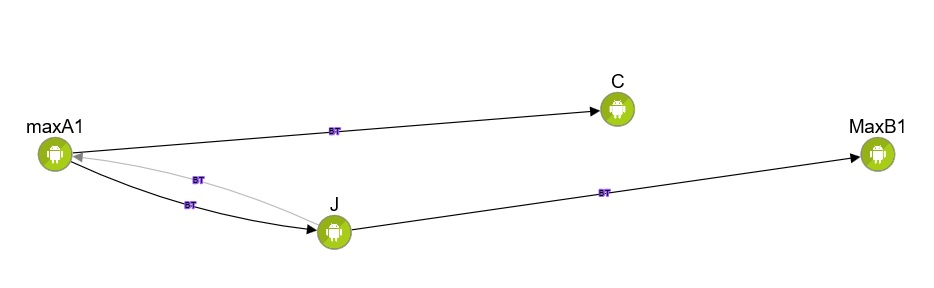
\includegraphics[width=1.0\textwidth]{belege/grosstests/Bilder/Miserfolg2.jpg}\\
5. Auch hier kommt die Nachricht nicht an Handy C vorbei. Auf einem
anderem Pfad schafft sie zwei Hops.\\
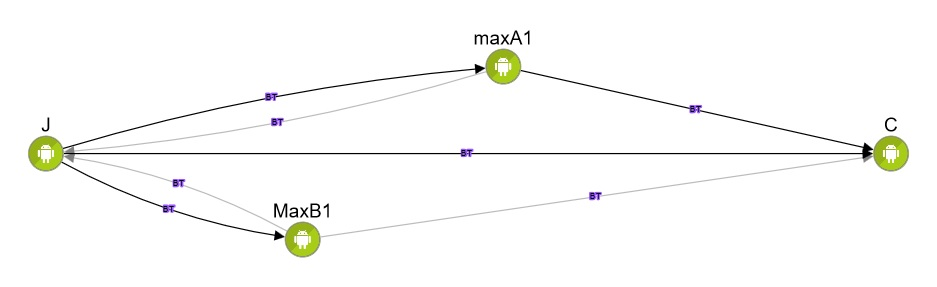
\includegraphics[width=1.0\textwidth]{belege/grosstests/Bilder/Miserfolg1.jpg}\\ 6. J versendet
hier die Nachricht an seine 3 Nachbarn. Da jedoch J, A und B (nur) C als
Nachbarn finden, kommt die Nachricht nicht an.\\\\

\clearpage\subsection{Schlussfolgerung aus dem
Test:}\label{schlussfolgerung-aus-dem-test}

Es kamen extrem wenige Nachrichten an. Dies lag daran, dass die Handys
Probleme hatten, sich zu verbinden. Es liegt nahe, dass der
Bluetoothadapter nicht genügend Ports hat um sich mit allen in der Nähe
befindlichen Geräten zu verbinden. Eine Möglichkeit dies zu lösen, wäre
es, sich nicht dauerhaft mit allen Geräten in der Umgebung zu verbinden,
sondern eine Verbindung nach einer Übertragung wieder zu schließen.

Des Weiteren gab es Handys, die Nachrichten überhaupt nicht
weitergeleitet haben. Vermutlich war an diesen der Stromsparmodus von
Android aktiv. Ein Beispiel hierfür wäre C.
\\\\
\textbf{Verbesserungen bis zum nächsten Test:}
\\\\
\begin{itemize}
\tightlist
\item
  Die Anzahl der aufzubauenden Verbindungen heruntersetzen.
\item
  Ein Test mit mehr anwesenden Personen durchführen um Android daran zu
  hindern in den Stromsparmodus zu gehen, da dieser nicht ohne
  Root-Rechte abschaltbar ist.
\end{itemize}

\clearpage\subsection{Ergebnisse Test 2:}\label{ergebnisse-test-2}

Bevor wir Test 2 gestartet haben, haben wir auf allen Handys den
Bluetooth Adapter deaktiviert und erneut aktiviert. Das sollte
eingefrorene Bluetooth Adapter wieder aktivieren. Dieses Vorgehen
basierte auf Erfahrungen von früheren kleinen Tests beim Programmieren.

Im Test 2 haben wir auf 166 Nachrichten 2 erfolgreiche Fälle und 164
Errors.

\textbf{Folgende Beispiele veranschaulichen die Nachrichten, die beim
Empfänger angekommen sind:}\\
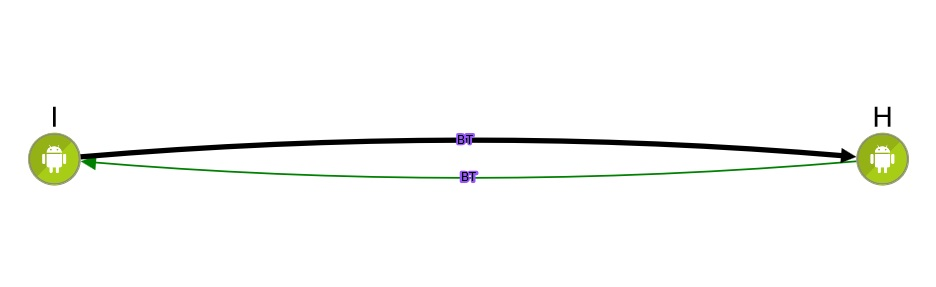
\includegraphics[width=1.0\textwidth]{belege/grosstests/Bilder/Test2Erfolg1.jpg}\\
 1. Nachricht
zwischen zwei benachbarten Handys.\\
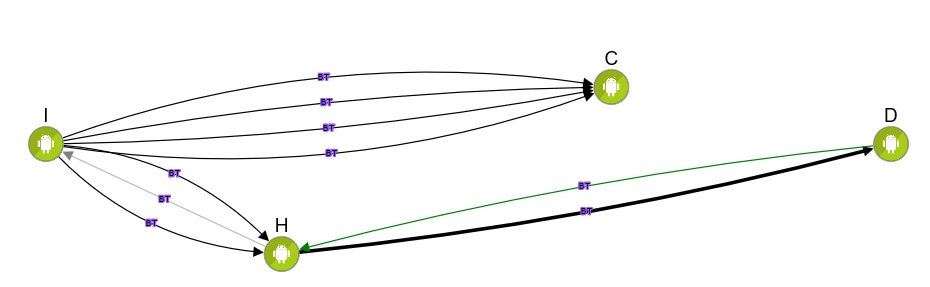
\includegraphics[width=1.0\textwidth]{belege/grosstests/Bilder/Test2Erfolg2.jpg}\\ 2. Nachricht
über einen Hop, die bei einem Retry erfolgreich wurde.\\

\textbf{Folgende Beispiele veranschaulichen Nachrichten, die nicht beim
Empfänger angekommen sind:}\\

\includegraphics[width=1.0\textwidth]{belege/grosstests/Bilder/Test2Misserfolg1.jpg}\\ 1. Das
Handy J hatte während des kompletten Tests keine Verbindung zu einem
Handy aufbauen können.\\
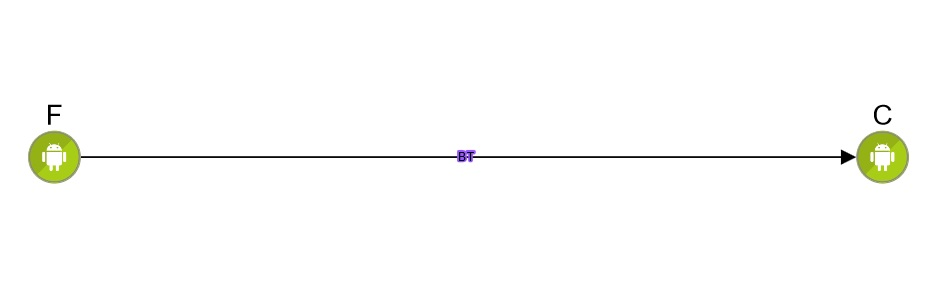
\includegraphics[width=1.0\textwidth]{belege/grosstests/Bilder/Test2Misserfolg3.jpg}\\ 2.
Generell hatten die Handys mehr Probleme Verbindungen aufzubauen.
Dadurch gab es viele Nachrichten, die gar nicht, oder nur bis zum
Nachbarn weitergeleitet wurden.\\
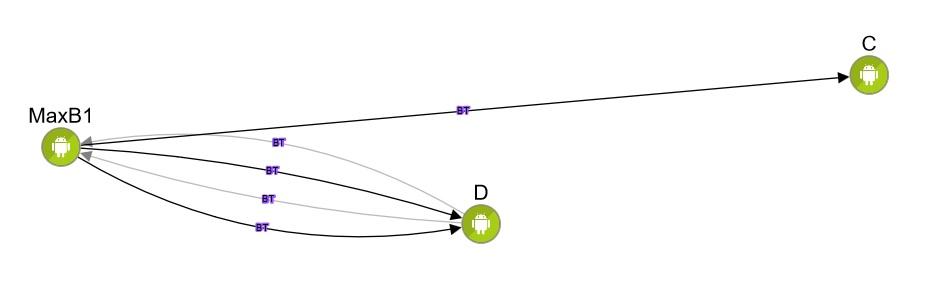
\includegraphics[width=1.0\textwidth]{belege/grosstests/Bilder/Test2Misserfolg4.jpg} \\3. Das
Handy B versucht eine Nachricht zu verschicken, schafft es jedoch nur
bis zu seinen unmittelbaren Nachbarn.\\
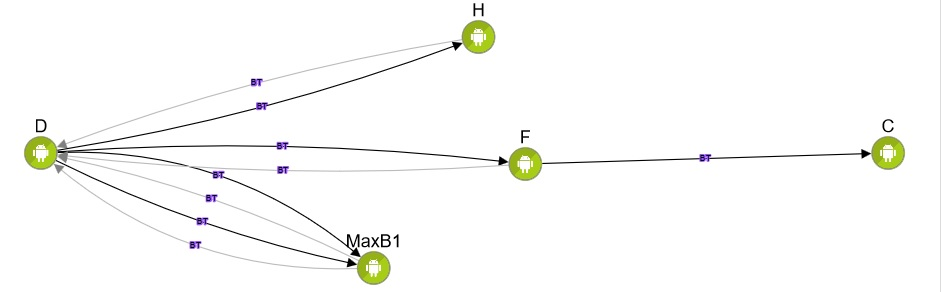
\includegraphics[width=1.0\textwidth]{belege/grosstests/Bilder/Test2Misserfolg5.jpg}\\
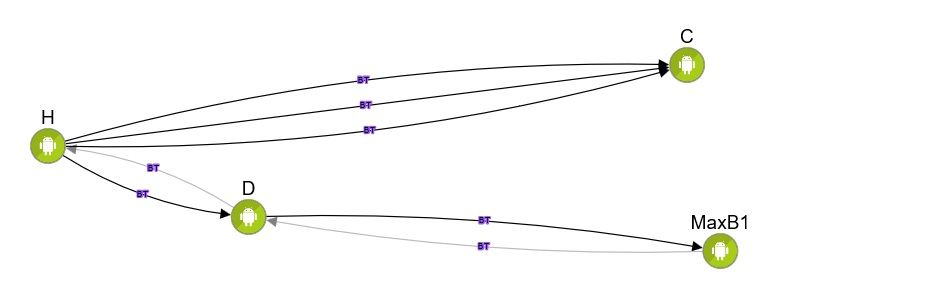
\includegraphics[width=1.0\textwidth]{belege/grosstests/Bilder/Test2Misserfolg6.jpg}\\ 4. und
5. Nachrichten wurden von einem Handy verschickt und schafften es eine
Nachricht mehr als einen Hop zu übertragen. Dies passierte bei diesem
Test bereits sehr selten.\\

\clearpage\subsection{Schlussfolgerung aus dem
Test:}\label{schlussfolgerung-aus-dem-test-1}

Dieser Test zeigte, dass bereits Abstände von circa 5 Metern einen stark
beeinflussenden Faktor haben und extrem viel weniger Verbindungen
aufgebaut wurden als in Test 1.\\\\

Auch hier gab es wieder Handys, die vermutlich von Android in den
Energiesparmodus versetzt wurden, da diese von niemandem bedient wurden
und nur als Relaisstadion gedient haben.

\textbf{Verbesserungen bis zum nächsten Test:}

siehe Test 1, keine weiteren Erkenntnisse gewonnen.

\clearpage\subsection{Test 3:}\label{test-3}

Da die Ergebnisse nicht unseren Erwartungen entsprachen, beschlossen wir
den Test hier abzubrechen. Der letzte Test unterliegt schwereren
Bedingungen und bringt dadurch nur bei Erfolg von Test 1 oder 2 bessere
Ergebnisse.

\clearpage\subsection{Testbericht}\label{testbericht-1}

Nach dem letzten Test wurde der Code so erweitert, dass Bluetooth nur
noch 4 Verbindungen gleichzeitig aufbaut und in regelmäßigen Abständen
alte Verbindungen fallen lässt. Das hindert den Bluetooth Adapter zu
schnell zu überlasten.\\\\

Außerdem wurden weitere Kommilitonen darum gebeten am Test teilzunehmen.
Insgesamt wurde der Test von 9 Personen mit 14 Handys ausgeführt.\\\\

Die Benennung der Handys wurde den einzelnen Personen überlassen. Es
wurde dafür gesorgt, dass alle Handys den Kontakt der anderen Handys
kennt.\\\\

\clearpage\subsection{Ergebnisse Test 1:}\label{ergebnisse-test-1-1}

Wir haben auf 167 Nachrichten 8 erfolgreiche Fälle und 159 Errors.

\textbf{Folgende Beispiele veranschaulichen Nachrichten, die beim
Empfänger angekommen sind:}\\
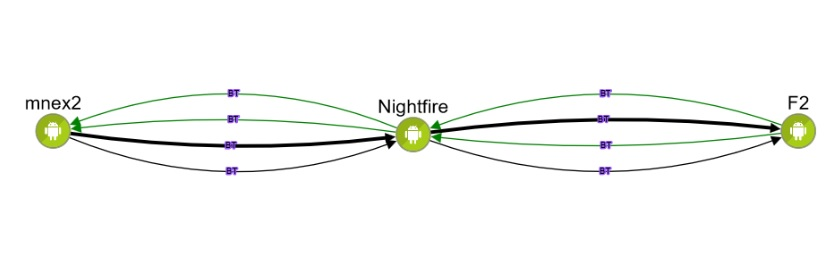
\includegraphics[width=1.0\textwidth]{belege/grosstests/Bilder/Grosstest2/Test1Erfolg2.jpg}\\
1. mnex2 sendet eine Nachricht an F2. Diese kommt erst nach einer
Retransmission an. Das Acknowledgement kommt auch erst beim 2. Versuch
an.\\
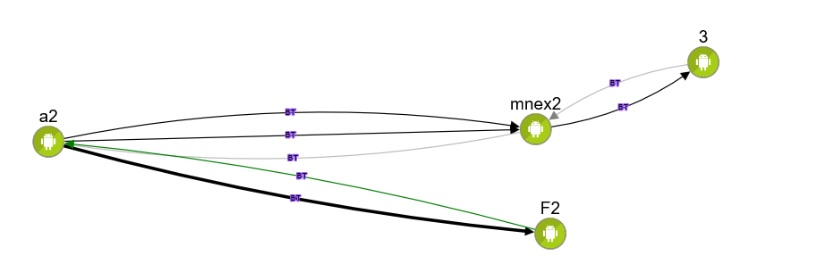
\includegraphics[width=1.0\textwidth]{belege/grosstests/Bilder/Grosstest2/Test1Erfolg1.jpg}\\
Hier sendet a2 eine Nachricht an F2. Da F2 ein Nachbar ist, kommt die
Nachricht direkt an. A2 versucht gleichzeitig auch noch einen weiteren
Weg, der jedoch nach einem Hop verloren geht.\\
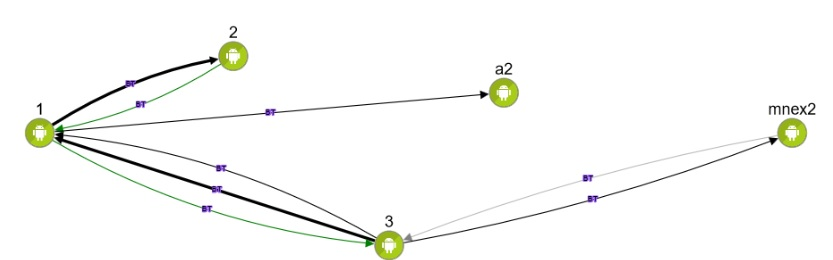
\includegraphics[width=1.0\textwidth]{belege/grosstests/Bilder/Grosstest2/Test1Erfolg3.jpg}\\
In dieser Nachricht sendet 3 an 2. Die Nachricht wird erfolgreich über 1
geschickt. 1 sendet die Nachricht gleichzeitig auch noch an a2.
\\
\textbf{Folgende Beispiele veranschaulichen Nachrichten, die nicht beim
Empfänger angekommen sind:}\\
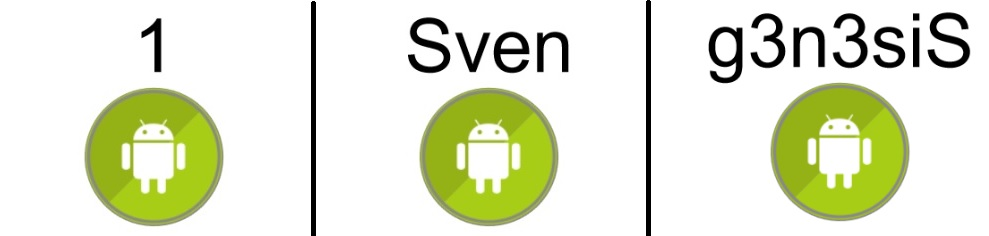
\includegraphics[width=1.0\textwidth]{belege/grosstests/Bilder/Grosstest2/Test1Misserfolg2.jpg}\\
Bei diesem Test kam es häufig zur Situation, dass Handys überhaupt keine
Verbindung mit anderen Geräten herstellen konnten. Dies kann daran
liegen, dass die Geräte in der Näheren Umgebung bereits 4 Verbindungen
offen hatten, oder dessen Bluetooth durch frühere Transmissions
überlastet war.\\

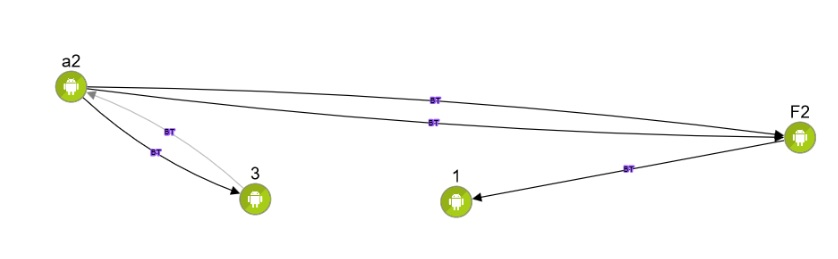
\includegraphics[width=1.0\textwidth]{belege/grosstests/Bilder/Grosstest2/Test1Misserfolg1.jpg}\\
Hier sendet a2 eine Nachricht, die jedoch nur über einen Hop
weitergeleitet wird und deshalb nicht ankommt.\\
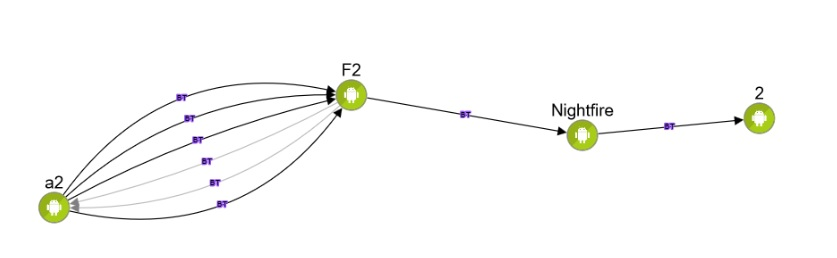
\includegraphics[width=1.0\textwidth]{belege/grosstests/Bilder/Grosstest2/Test1Misserfolg3.jpg}\\
Auch hier sendet a2 eine Nachricht, die über die Hops F2, Nightfire und
2 läuft, dort jedoch verloren geht.\\

\clearpage\subsection{Schlussfolgerung aus dem
Test:}\label{schlussfolgerung-aus-dem-test-2}

Die Einschränkung auf 4 Verbindungen pro Bluetooth-Gerät scheint nicht
erfolgreich gewesen zu sein. Der Bluetoothadapter scheint immer noch
sehr schnell zu überlasten. Die Einschränkung führt außerdem noch dazu,
dass nicht alle Handys in der Umgebung erreicht werden, da bereits 4
Verbindungen bestehen, oder versucht aufgebaut zu werden.\\\\

Es bestand kein Grund zur Annahme, dass Verbindungen bei diesem Test
nicht zustande gekommen sind, weil ein Handy in den Standby Modus
gegangen ist.

\clearpage\subsection{Ergebnisse Test 2:}\label{ergebnisse-test-2-1}

Wir haben auf 227 Nachrichten 20 erfolgreiche Fälle und 7 Errors.\\\\

\textbf{Folgende Beispiele veranschaulichen Nachrichten, die beim
Empfänger angekommen sind:}\\\\
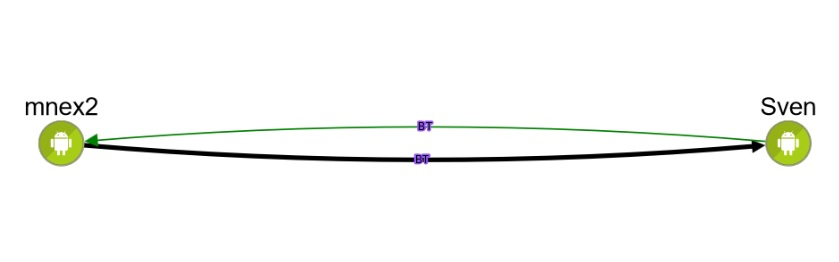
\includegraphics[width=1.0\textwidth]{belege/grosstests/Bilder/Grosstest2/Test2Erfolg1.jpg}\\
Die Verbindung zwischen mnex2 und Sven bestand über den ganzen Test.
Über diese Verbindung gingen 13 Nachrichten.\\
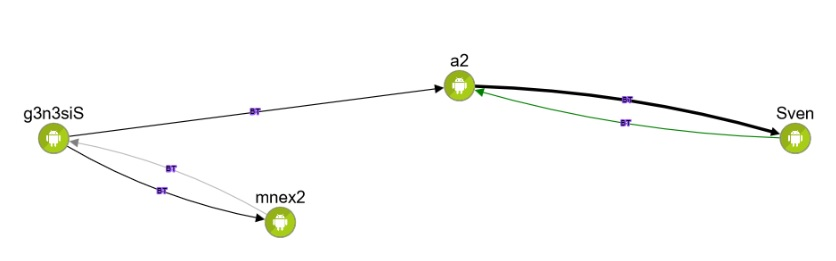
\includegraphics[width=1.0\textwidth]{belege/grosstests/Bilder/Grosstest2/Test2Erfolg3.jpg}\\
G3n3siS sendet eine Nachricht an Sven. Diese wird erfolgreich an a2
übermittelt, welches diese dann an Sven weiterleitet. Das
Acknowledgement kommt jedoch nicht mehr zurück.\\
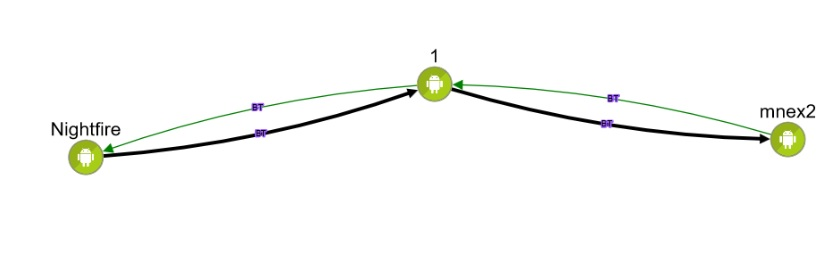
\includegraphics[width=1.0\textwidth]{belege/grosstests/Bilder/Grosstest2/Test2Erfolg4.jpg}\\
Nightfire sendet eine Nachricht an mnex2.\\

\textbf{Folgende Beispiele veranschaulichen Nachrichten, die nicht beim
Empfänger angekommen sind:}\\

\includegraphics[width=1.0\textwidth]{belege/grosstests/Bilder/Grosstest2/Test2Misserfolg1.jpg}\\
Im Verhältnis zu Test 1 gab es noch häufiger die Situation, dass Handys
gar nicht mit anderen Geräten verbunden sind.\\
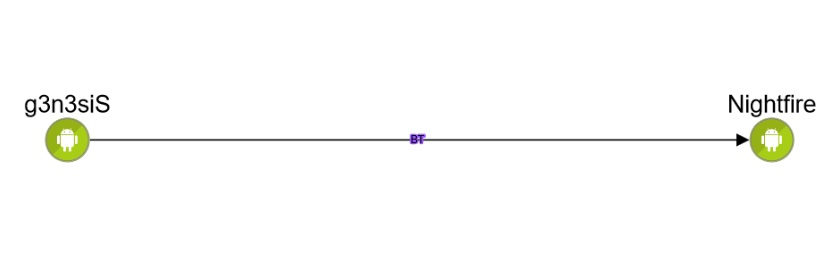
\includegraphics[width=1.0\textwidth]{belege/grosstests/Bilder/Grosstest2/Test2Misserfolg2.jpg}\\
G3n3siS verschickt eine Nachricht, die jedoch von seinem Nachbarn
Nightfire nicht weitergeleitet wird.\\
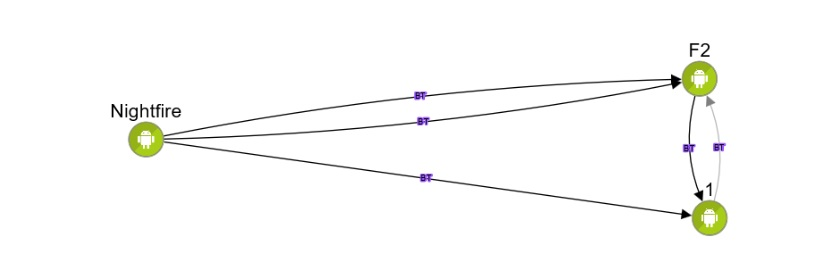
\includegraphics[width=1.0\textwidth]{belege/grosstests/Bilder/Grosstest2/Test2Misserfolg3.jpg}\\
Nightfire baut eine Verbindung zu mehreren Nachbargeräten auf, die sich
jedoch nur gegenseitig finden.\\

\clearpage\subsection{Schlussfolgerung aus dem
Test:}\label{schlussfolgerung-aus-dem-test-3}

Die Anzahl der erfolgreichen Verbindungen ist sehr stark von der
funktionierenden Verbindung zwischen mnex und Sven beeinflusst.\\\\

Die Tatsache, dass extrem viele Geräte überhaupt keine Verbindung mehr
aufbauen konnten, unterstützt die Aussage, die bereits nach Test 1
getroffen wurde, dass die Limitierung der Slots nicht zielführend war.

\clearpage\subsection{Ergebnisse Test 3:}\label{ergebnisse-test-3}

Da wir gemerkt haben, dass die Limitierung der Slots auf 3 nicht
zielführend war, haben wir diese für Test 3 wieder rückgängig gemacht.\\\\

Wir haben auf 164 Nachrichten 11 erfolgreiche Fälle und 153 Errors.
\\
\textbf{Folgende Beispiele veranschaulichen Nachrichten, die beim
Empfänger angekommen sind:}\\
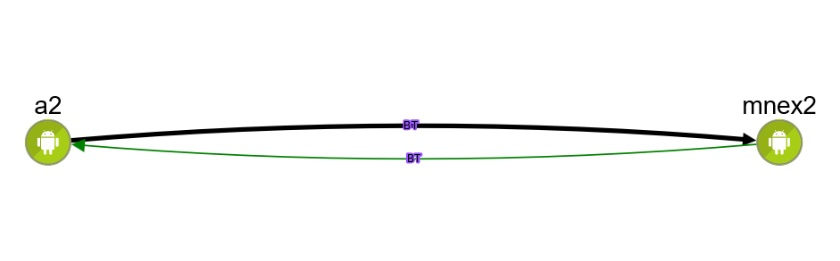
\includegraphics[width=1.0\textwidth]{belege/grosstests/Bilder/Grosstest2/Test3Erfolg1.jpg}\\
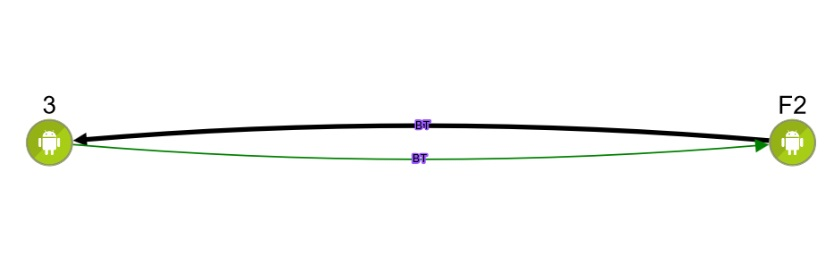
\includegraphics[width=1.0\textwidth]{belege/grosstests/Bilder/Grosstest2/Test3Erfolg2.jpg}\\
Nachrichten die zu einem benachbarten Empfänger gesendet werden.\\
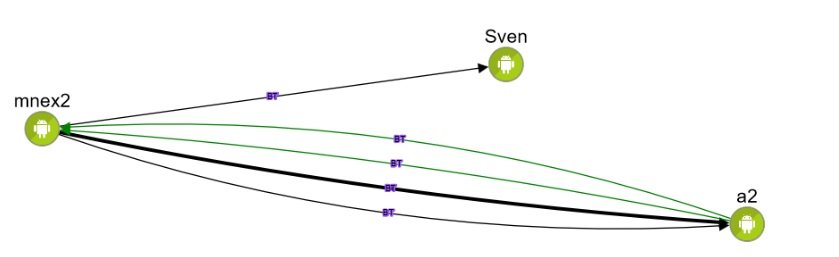
\includegraphics[width=1.0\textwidth]{belege/grosstests/Bilder/Grosstest2/Test3Erfolg3.jpg}\\

Mnex sendet eine Nachricht an Sven diese kommt jedoch erst nach dem
zweiten Versuch an. Auch das Acknowledgement benötigt 2 Versuche.
\\
\textbf{Folgende Beispiele veranschaulichen Nachrichten, die nicht beim
Empfänger angekommen sind:}\\

\includegraphics[width=1.0\textwidth]{belege/grosstests/Bilder/Grosstest2/Test3Misserfolg1.jpg}\\
G3n3siS sendet eine Nachricht. Diese geht jedoch nach 2 Hops verloren.\\

\includegraphics[width=1.0\textwidth]{belege/grosstests/Bilder/Grosstest2/Test3Misserfolg2.jpg}\\
Das wohl häufigste Beispiel des dritten Tests. 2 Benachbarte Geräte
schaffen es eine Verbindung aufzubauen. Das zweite Handy schafft es
jedoch dann nicht, die Nachricht weiterzuleiten.\\


\includegraphics[width=1.0\textwidth]{belege/grosstests/Bilder/Grosstest2/Test3Misserfolg3.jpg}\\
Auch hier gab es Fälle, in denen ein Handy keine Verbindung mit einem anderen Gerät aufbauen konnte. Dies passiert jedoch deutlich seltener als bei Test 1 und 2. 
\clearpage\subsection{Schlussfolgerung aus dem
Test:}\label{schlussfolgerung-aus-dem-test-4}

Der dritte Test ist besser gelaufen als der 2. Da die Entfernung einen
erschwerenden Faktor darstellt, kann davon ausgegangen werden, dass die
Verbesserung dadurch zustande kam, dass wir die Slots nicht mehr
limitieren.

\clearpage\subsection{Ausblick und zukünftige
Tests:}\label{ausblick-und-zukuxfcnftige-tests}

Im Auftragsgebertreffen wurde entschieden, dass keine weiteren
Verbesserungen am Code durchgeführt werden sollen. Die Begründung
hierfür ist, dass die Implementierung des Bluetooth Stacks wohl
teilweise fehlerhaft ist.
\\\\
Die Lösung hierfür ist eine eigene Implementierung des Bluetooth Stacks.
Diese soll jedoch im Rahmen einer Bachelorarbeit geschrieben werden, da
dies nicht Bestandteil des Bachelorpraktikums ist.
\\\\
Da sich deshalb in der Funktionalität der Nachrichtenübertragung nichts
mehr ändern wird, haben wir auf den dritten Großtest verzichtet.





\end{document}
